\documentclass{article}

% Definitions
\newcommand{\pavo}{{\tt pavo}}  % you can use \pavo{} to print pavo as package
\newcommand{\code}[1]{{\tt #1}}  % way to plot out code
\setlength{\parindent}{0in}
\setlength{\parskip}{.1in}
\setlength{\textwidth}{140mm}
\setlength{\oddsidemargin}{10mm}
\usepackage{amsmath}
\usepackage{cite}

\usepackage{Sweave}
\begin{document}

\Sconcordance{concordance:pavo.tex:pavo.rnw:%
1 12 1 1 0 3 1 1 7 80 1 1 2 4 0 1 2 15 1}



\title{\pavo{}: {\bf P}erceptual {\bf A}nalysis, {\bf V}isualization and {\bf O}rganization of Color Data in R}
\author{Rafael Maia, Paul-Pierre Bitton, Chad Eliason}

\maketitle

\section*{Introduction}

Although \pavo{} deals largely with spectral reflectance data from bird feathers, it is meant 
to be applicable for a range of taxa. It provides flexible ways to input spectral data from a
variety of equipment manufacturers, process these data and...

\pavo{} was written with the following workflow in mind:

% numbered list of things
\begin{enumerate}
\item {\bf O}rganize spectral data by inputting files, processing spectra (e.g., to remove
noise, negative values, smooth curves, etc.)
\item {\bf A}nalyze the resulting files, either using typical tristimulus color variables (hue,
saturation, brightness) or using visual models based on perceptual data from the taxon of interest.
\item {\bf V}isualize the output
\end{enumerate}


\section{Organizing and Processing Spectral Data}

blah blah blah


\section{Analyzing Spectral Data}

\subsection{Overview}

add description here

\subsection{Variables calculated}

% A table for filling in Montgomerie's color variables
\begin{table}[h]
\begin{center}
\begin{tabular}{l l l} \hline
{\bf Color} & \\
{\bf Variable} & {\bf Equation} & {\bf Description} \\ 
\hline
\code{B1} & {$\sum_{\lambda={300}}^{700} R_\lambda$} & \parbox[t]{3in}{Total brightness, total reflectance}  \\
\code{B2} & {$B_\text{1}/n_\text{wl}$} & \parbox[t]{3in}{Mean brightness.} \\
\code{B3} & {$R_\text{max}$} & \parbox[t]{3in}{Intensity.} \\
\code{S1} & {} & \parbox[t]{3in}{Chroma, spectral purity.} \\
\code{S2} & {$R_\text{max}/R_\text{min}$} & \parbox[t]{3in}{Spectral saturation} \\
\code{S3} & {} & \parbox[t]{3in}{} \\
\code{S4} & {} & \parbox[t]{3in}{} \\
\code{S5} & {} & \parbox[t]{3in}{} \\
\code{S6} & {} & \parbox[t]{3in}{} \\
\code{S7} & {} & \parbox[t]{3in}{} \\
\code{S8} & {} & \parbox[t]{3in}{} \\
\code{S9} & {} & \parbox[t]{3in}{} \\
\code{S10} & {} & \parbox[t]{3in}{} \\
\code{H1} & {$\lambda_\text{Rmax}$} & \parbox[t]{3in}{Hue: wavelength of peak reflectance} \\
\code{H2} & {} & \parbox[t]{3in}{} \\
\code{H3} & {} & \parbox[t]{3in}{} \\
\code{H4} & {} & \parbox[t]{3in}{} \\
\code{H5} & {} & \parbox[t]{3in}{} \\
\hline
\end{tabular}
\end{center}
\caption{\label{table:tristim}
The complete set of tristimulus variables calculated by \code{summary} in \pavo{}}
\end{table}

Color variables described in Table \ref{table:tristim}.

blah blah blah\footnote{some footnote text here} and also this.

\section{Visualizing Spectral Data}




\section*{Examples}


\begin{Schunk}
\begin{Sinput}
> hist(rnorm(50))
\end{Sinput}
\end{Schunk}

\begin{figure}[h] % h=here, t=top, b=bottom, p=floating page
\begin{center}
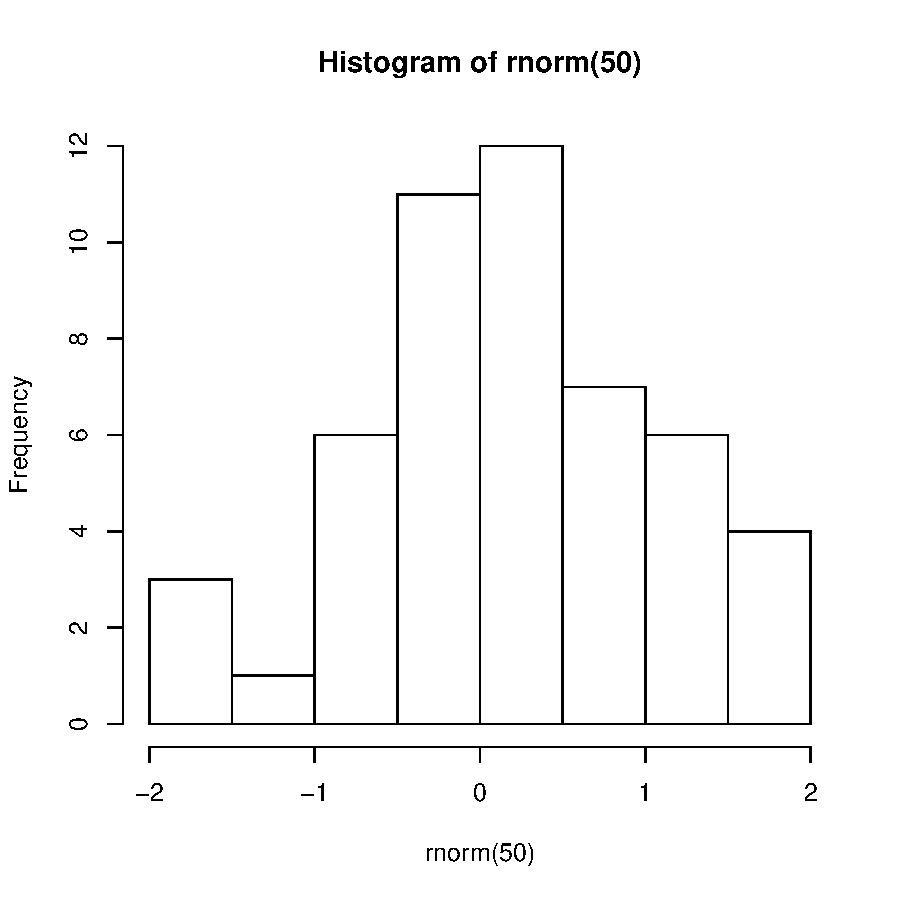
\includegraphics[width=5in]{pavo-fig1}
\end{center}
\caption{Sample plot.}
\label{fig1}
\end{figure}

\subsection*{More examples}

Some more examples:

\bibliography{}

\end{document}
